%\chapter{Wireless IoT Protocols} 
There are several wireless protocols commonly used in IoT (Internet of Things) devices to enable wireless communication. In the realm of wireless IoT, a diverse range of wireless communication methods and protocols, such as Internet Protocol Version 6 (IPv6), low-power Wireless Personal Area Network (6LoWPAN), Bluetooth Low Energy (BLE), Z-Wave, ZigBee, LTE-M, and LoRa can be harnessed to establish connections with smart devices \cite{IoT_Protocol}. We have discussed about some IoT protocols below:

\section{Wi-Fi}
Wi-Fi is a widely used wireless communication protocol that allows IoT devices to connect to the internet and other devices within a local area network (LAN). It offers high data rates and is suitable for applications that require high bandwidth, such as video streaming or cloud connectivity. A collection of wireless LAN (WLAN) protocols is known as IEEE 802.11. It has through several versions, including 802.11b, 802.11a, 802.11g, 802.11n, 802.11ac, 802.11ah, and 802.11ax before becoming the 802.11be.

\section{Bluetooth}
Bluetooth is a short-range wireless protocol used for connecting IoT devices over short distances. It is commonly used for applications like home automation, wearable devices, and personal health monitoring. Bluetooth Low Energy (BLE) is a power-efficient variant of Bluetooth designed for IoT devices with limited power resources. Since its inception in version 2.0, Bluetooth has undergone several generations, from the debut of low power (LE) in version 4.0 to the present version 5.3. Version 5.0 of BLE has a coverage range of up to 400 m, compared to version 4.0's 100 m.

\section{Zigbee}
 Zigbee is a low-power, low-data-rate wireless protocol designed for home automation and industrial control applications. It supports mesh networking, allowing IoT devices to create self-forming and self-healing networks. Zigbee is known for its low power consumption, making it suitable for battery-powered devices.
\section{Z-Wave}
A more recent kind of RF called Z-Wave is suitable for short-range wireless communication systems because it is affordable, uses little energy, is accurate, and is all of the above. It is another wireless protocol used primarily in home automation systems. It operates in the sub-GHz frequency range, providing good range and penetration through walls. Z-Wave is designed to minimize interference between devices and supports mesh networking for extended coverage.
\section{Thread}
Thread is an IP-based wireless protocol built on the IEEE 802.15.4 standard. It provides secure, reliable, and low-power connectivity for IoT devices. Thread is designed for smart home applications and supports mesh networking, allowing devices to communicate with each other and create a network with improved coverage and redundancy.
\section{LoRaWAN}
 LoRaWAN (Long Range Wide Area Network) is a low-power, wide-area network protocol designed for long-range communication. It operates in unlicensed frequency bands, offering excellent coverage and long battery life for IoT devices. LoRaWAN is often used in applications such as smart cities, agriculture, and asset tracking. Small payloads, such as data from sensors, may be sent over great distances with LoRaWAN. Additionally, it offers coverage up to 25 miles away in line of sight or 800 meters through structures. As a security measure, it primarily uses the 128-bit symmetrical Advanced Encryption Standard (AES) encryption. Compared to other wireless data transmission systems, this provides a significantly greater communication range while keeping low bandwidths.

\section{NB-IoT}
 NB-IoT and LTE-M are cellular network technologies designed specifically for IoT applications. They provide wide coverage, strong security, and support for a large number of devices. There are 3 main operational modes for NB-IoT. When using the in-band option, the narrowband is utilized inside an LTE carrier. The Guardband mode enables NB-IoT to utilize the extra bandwidth on LTE. The narrowband is utilized in its own frequency band in the standalone mode. NB-IoT and LTE-M are suitable for applications that require mobility or operate in areas without Wi-Fi coverage.
\section{Wi-SUN}
(Wireless Smart Utility Network) stands for a wireless communication technology specifically designed for large-scale, outdoor industrial and utility applications. It's designed to provide reliable, secure, and long-range communication for applications such as smart meters, smart street lighting, and other industrial IoT (Internet of Things) deployments. According to the area, the Wi-SUN mesh computing protocol uses the 800 MHz, 900 MHz, and 2.4 GHz band frequencies and provides communication in both directions.

\section{Performance map of wireless protocols}
The distance coverage, speeds, ranges, and power consumption of several wireless communication technologies are compared in Figure \ref{fig:x Performance MAP}.

\begin{figure}[htbp]
\centering
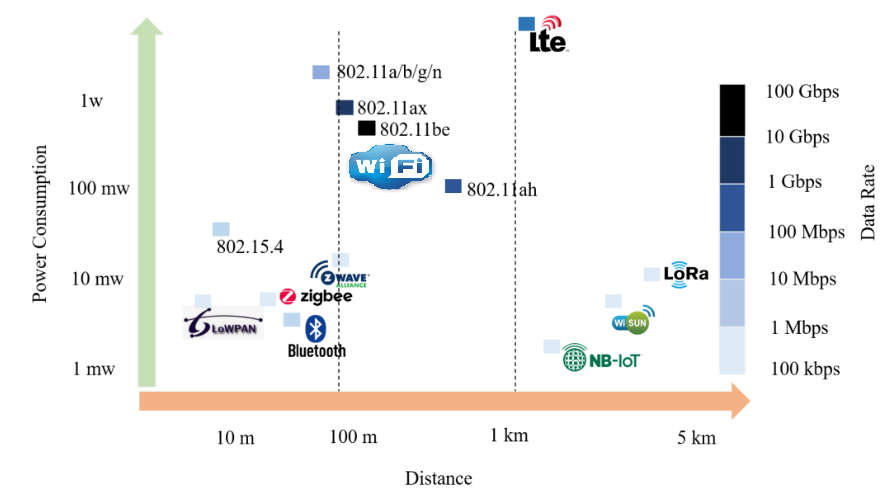
\includegraphics[scale=0.9]{images/PerformanceMap.png}
\caption{Power consumption, coverage distance, and data rate for the different protocols.}
\label{fig:x Performance MAP}
\end{figure}
The choice of wireless protocol depends on factors such as range, data rate, power consumption, latency, scalability, security, cost, deployment environment, and application requirements \cite{PerformanceMAP}. Each protocol is designed to address specific use cases, and selecting the right one involves evaluating these factors to meet the demands of your IoT deployment. After analysing all the parameters, requirements, and studying the LTE-M System Performance from \cite{LTE-M_Perform}, we have chosen NB-IoT protocol for our acquisition system.

\nomenclature{$IoT$}{Internet of Things}
\nomenclature{$LAN$}{Local Area Network}
\nomenclature{$BLE$}{Bluetooth Low Energy}
\nomenclature{$LoRaWAN$}{Long Range Wide Area Network}
\nomenclature{$NB-IoT$}{Narrowband IoT}
\nomenclature{$LTE-M$}{Long Term Evolution Machine Type Communication}
\nomenclature{$AES$}{Advanced Encryption Standard}
\nomenclature{$Wi-SUN$}{Internet of Things}
\nomenclature{$WiFi$}{Wireless Smart Utility Network}



